% ============================== CHAPTER 5 ==============================
\chapterdivider{5}{CONCLUSION}
\chapter{Conclusion}

\section{Limitations}
\begin{itemize}
\item \textbf{Model, not the authors' simulation.} The OMNeT++ network is our model of the environment stated in Table~II of~\cite{base}; the authors' simulation is not available. The adversary rate, the authentication window and the enrolment rule are our assumptions. The saturated latencies of the scanning strategies depend on them, but the ranking does not (Table~\ref{tab:sens}); apart from the runs with and without adversaries, that analysis uses the offered load of the mean server rather than new simulation runs.
\item \textbf{No hardware timings.} Every probe is priced with the paper's constant $T_H=0.32$\,ms. The ESP8266 port demonstrates that the device side runs on real hardware, but the reported latencies are not measured on it.
\item \textbf{Partial modelling of two strategies.} CR and MW change the first message and are modelled at the resolution level only.
\item \textbf{One point on each trade-off.} The TM parameters (six tables, $m=128$) and the window parameters ($L=16$, $F=8$, $W_t=3$) are single choices; other choices move each strategy along its curve.
\item \textbf{Our reading of the specification.} Epoch semantics, windows and tables are our choices, and conformance means agreement with our reading of Section~III, which only the authors can confirm.
\item \textbf{Symbolic verification only.} The ProVerif results assume perfect primitives and do not include the server's replay state, so injective device authentication (Q4) is checked by test rather than proved.
\item \textbf{Prototype scope.} Devices are static, coverage is an abstract predicate, re-keying is a stub, the key store is demonstration-grade, and side channels are out of scope.
\end{itemize}

\section{Conclusion}
A server cannot authenticate a device that it has not yet identified. In the two-message protocol of Al-Rasheed et al.~\cite{base}, that identification, pseudonym resolution, is a required step with no specification and no cost in the model. This project showed from the specification alone that every correct server must perform it, implemented the protocol in Python and on the device side in C with byte-for-byte conformance to independent vectors, and compared seven ways of filling the gap under the paper's own constants and network.

The choice turned out to decide the protocol's practical behaviour. With a precomputed table (O2) the server stays within 1\,ms of the published 23.68\,ms per session at 1,000 devices and rejects forged pseudonyms for free, at a memory cost of tens of kilobytes per server. With the on-demand counter scan that the specification suggests (O1), the session latency reaches about 44\,s at the same scale with 5\% adversaries, forged pseudonyms are an effective denial-of-service attack that the block-list never sees, and an attacker who drops $F$ consecutive messages ($F=8$ in our configuration) locks a device out for good. This ranking holds under every assumption we varied, although the size of the slowdown depends on them. Clock epochs avoid the lockout but make sessions in one epoch linkable. The formal analysis shows that the protocol's secrecy and agreement properties do not depend on the choice, whereas unlinkability and injective authentication do, and that the protocol has no forward secrecy.

All seven objectives of the project were achieved. The practical recommendation is that a deployment with counter epochs should precompute (O2) and add a resynchronisation path, that a deployment with clocks can use O4 if it accepts linkability within an epoch and keeps a nonce cache, and that the specification should state the epoch semantics, the resolution method and the replay state, and add a resolution term to its cost model. Precomputed tables, the oldest answer from RFID private identification, keep the protocol's cost claim intact.

\section{Future Scope}
\begin{itemize}
\item \textbf{Stateful verification.} Prove injective device authentication with the replay window included, for example in Tamarin, which supports mutable state.
\item \textbf{Hardware measurements.} Measure resolution and handshake times on the ESP8266 and on a server-class machine, and replace the paper's $T_H$ constant with measured values.
\item \textbf{Resynchronisation.} Design and verify a recovery path for counter epochs after the lockout, and study the trade-off between a larger forward window $F$ and table size.
\item \textbf{Full handshakes for CR and MW.} Integrate the strategies that change $M_1$ into the full exchange and the simulator, and quantify MW's privacy loss under device compromise.
\item \textbf{Broader parameter sweeps.} Explore the TM trade-off curve, epoch lengths for O4, adversary rates, mobility and hand-off.
\item \textbf{Re-keying and forward secrecy.} Implement the TA-assisted re-keying of Eq.~24 and evaluate extensions that add forward secrecy.
\item \textbf{Other protocols.} Apply the same method, i.e.\ derive the resolution step from the specification, measure it, and price it under the paper's own constants, to other pseudonym-based IoT authentication schemes.
\end{itemize}

% ============================== REFERENCES ==============================
\clearpage
\phantomsection
\addcontentsline{toc}{chapter}{References}
\renewcommand{\bibname}{References}
\begin{thebibliography}{99}
\bibitem{base} A. Al-Rasheed, R. Khan, A. Ahmad, A. Saeed, F. Alturise and S. Alkhalaf, ``A low-cost hybrid elliptic curve cryptography authentication protocol for trustworthy Internet of Things communication,'' \emph{IEEE Trans. Consum. Electron.}, vol.~72, no.~2, pp.~4483--4491, May 2026, doi:10.1109/TCE.2026.3662053.
\bibitem{weis} S. A. Weis, S. E. Sarma, R. L. Rivest and D. W. Engels, ``Security and privacy aspects of low-cost radio frequency identification systems,'' in \emph{Security in Pervasive Computing (SPC 2003)}, LNCS 2802. Springer, 2004, pp.~201--212.
\bibitem{ohkubo} M. Ohkubo, K. Suzuki and S. Kinoshita, ``Cryptographic approach to `privacy-friendly' tags,'' in \emph{RFID Privacy Workshop}, MIT, Cambridge, MA, USA, Nov. 2003.
\bibitem{molnar} D. Molnar and D. Wagner, ``Privacy and security in library RFID: Issues, practices, and architectures,'' in \emph{Proc. 11th ACM Conf. Computer and Communications Security (CCS)}, 2004, pp.~210--219.
\bibitem{avoine05} G. Avoine and P. Oechslin, ``A scalable and provably secure hash-based RFID protocol,'' in \emph{Proc. 3rd IEEE Int. Conf. Pervasive Computing and Communications Workshops (PerCom Workshops)}, 2005, pp.~110--114.
\bibitem{ado05} G. Avoine, E. Dysli and P. Oechslin, ``Reducing time complexity in RFID systems,'' in \emph{Selected Areas in Cryptography (SAC 2005)}, LNCS 3897. Springer, 2006, pp.~291--306.
\bibitem{tsudik} G. Tsudik, ``YA-TRAP: Yet another trivial RFID authentication protocol,'' in \emph{Proc. 4th IEEE Int. Conf. Pervasive Computing and Communications Workshops (PerCom Workshops)}, 2006, pp.~640--643.
\bibitem{hellman} M. E. Hellman, ``A cryptanalytic time-memory trade-off,'' \emph{IEEE Trans. Inf. Theory}, vol.~26, no.~4, pp.~401--406, 1980.
\bibitem{oechslin} P. Oechslin, ``Making a faster cryptanalytic time-memory trade-off,'' in \emph{Advances in Cryptology -- CRYPTO 2003}, LNCS 2729. Springer, 2003, pp.~617--630.
\bibitem{omnet} A. Varga and R. Hornig, ``An overview of the OMNeT++ simulation environment,'' in \emph{Proc. SIMUTools}, 2008.
\bibitem{hkdf} H. Krawczyk and P. Eronen, ``HMAC-based extract-and-expand key derivation function (HKDF),'' RFC 5869, 2010.
\bibitem{fips180} National Institute of Standards and Technology, ``Secure hash standard (SHS),'' FIPS PUB 180-4, 2015.
\bibitem{gcm} M. Dworkin, ``Recommendation for block cipher modes of operation: Galois/Counter Mode (GCM),'' NIST SP 800-38D, 2007.
\bibitem{proverif} B. Blanchet, ``Modeling and verifying security protocols with the applied pi calculus and ProVerif,'' \emph{Foundations and Trends in Privacy and Security}, vol.~1, no.~1--2, pp.~1--135, 2016.
\bibitem{blanchet08} B. Blanchet, M. Abadi and C. Fournet, ``Automated verification of selected equivalences for security protocols,'' \emph{J. Log. Algebr. Program.}, vol.~75, no.~1, pp.~3--51, 2008.
\bibitem{arapinis} M. Arapinis, T. Chothia, E. Ritter and M. Ryan, ``Analysing unlinkability and anonymity using the applied pi calculus,'' in \emph{Proc. 23rd IEEE Computer Security Foundations Symp. (CSF)}, 2010, pp.~107--121.
\bibitem{repo} J. Kerkar, C. Kelkar, C. Poornamath, Y. Kolekar and S. Sondur, ``hybrid-ecc-iot-auth: Implementation, models and data for pseudonym resolution in two-message IoT authentication,'' 2026. [Online]. Available: \url{https://github.com/jaykerkar0405/hybrid-ecc-iot-auth}
\bibitem{apple} Apple, ``MacBook Pro (14-inch, 2023) -- Tech Specs,'' Apple Support. [Online]. Available: \url{https://support.apple.com/en-am/111340}
\end{thebibliography}

% ============================== APPENDIX ==============================
\clearpage
\chapter*{Appendix}
\addcontentsline{toc}{chapter}{Appendix}

\section*{A.I. Publication Details}
\addcontentsline{toc}{section}{A.I. Publication Details}
\textbf{Paper:} J.~Kerkar, C.~Kelkar, C.~Poornamath, Y.~Kolekar and S.~Sondur, ``Pseudonym Resolution and Formal Verification of an Unlinkable Two-Message IoT Authentication Protocol,'' 2026. Department of Information Technology, Vivekanand Education Society's Institute of Technology, Mumbai. Source and PDF: \texttt{paper/} in the project repository~\cite{repo}.

\textbf{Status:} Publication in progress. Venue, submission and acceptance details will be added when available.

\subsection*{Camera Ready / Published Paper}
\begin{center}
\fbox{\parbox{0.88\textwidth}{\centering\vspace{12pt}
Camera-ready / published paper and presentation certificate\\[6pt]
\textit{Reserved for the final documents when available.}\vspace{12pt}}}
\end{center}

\subsection*{Plagiarism report}
The project paper was checked for similarity using Turnitin (Submission ID 3089310696, 14~November 2026). The overall similarity index is \textbf{3\%}, made up of 2\% internet sources, 1\% publications and 1\% student papers. The matched sources are listed in the report reproduced on the following pages.

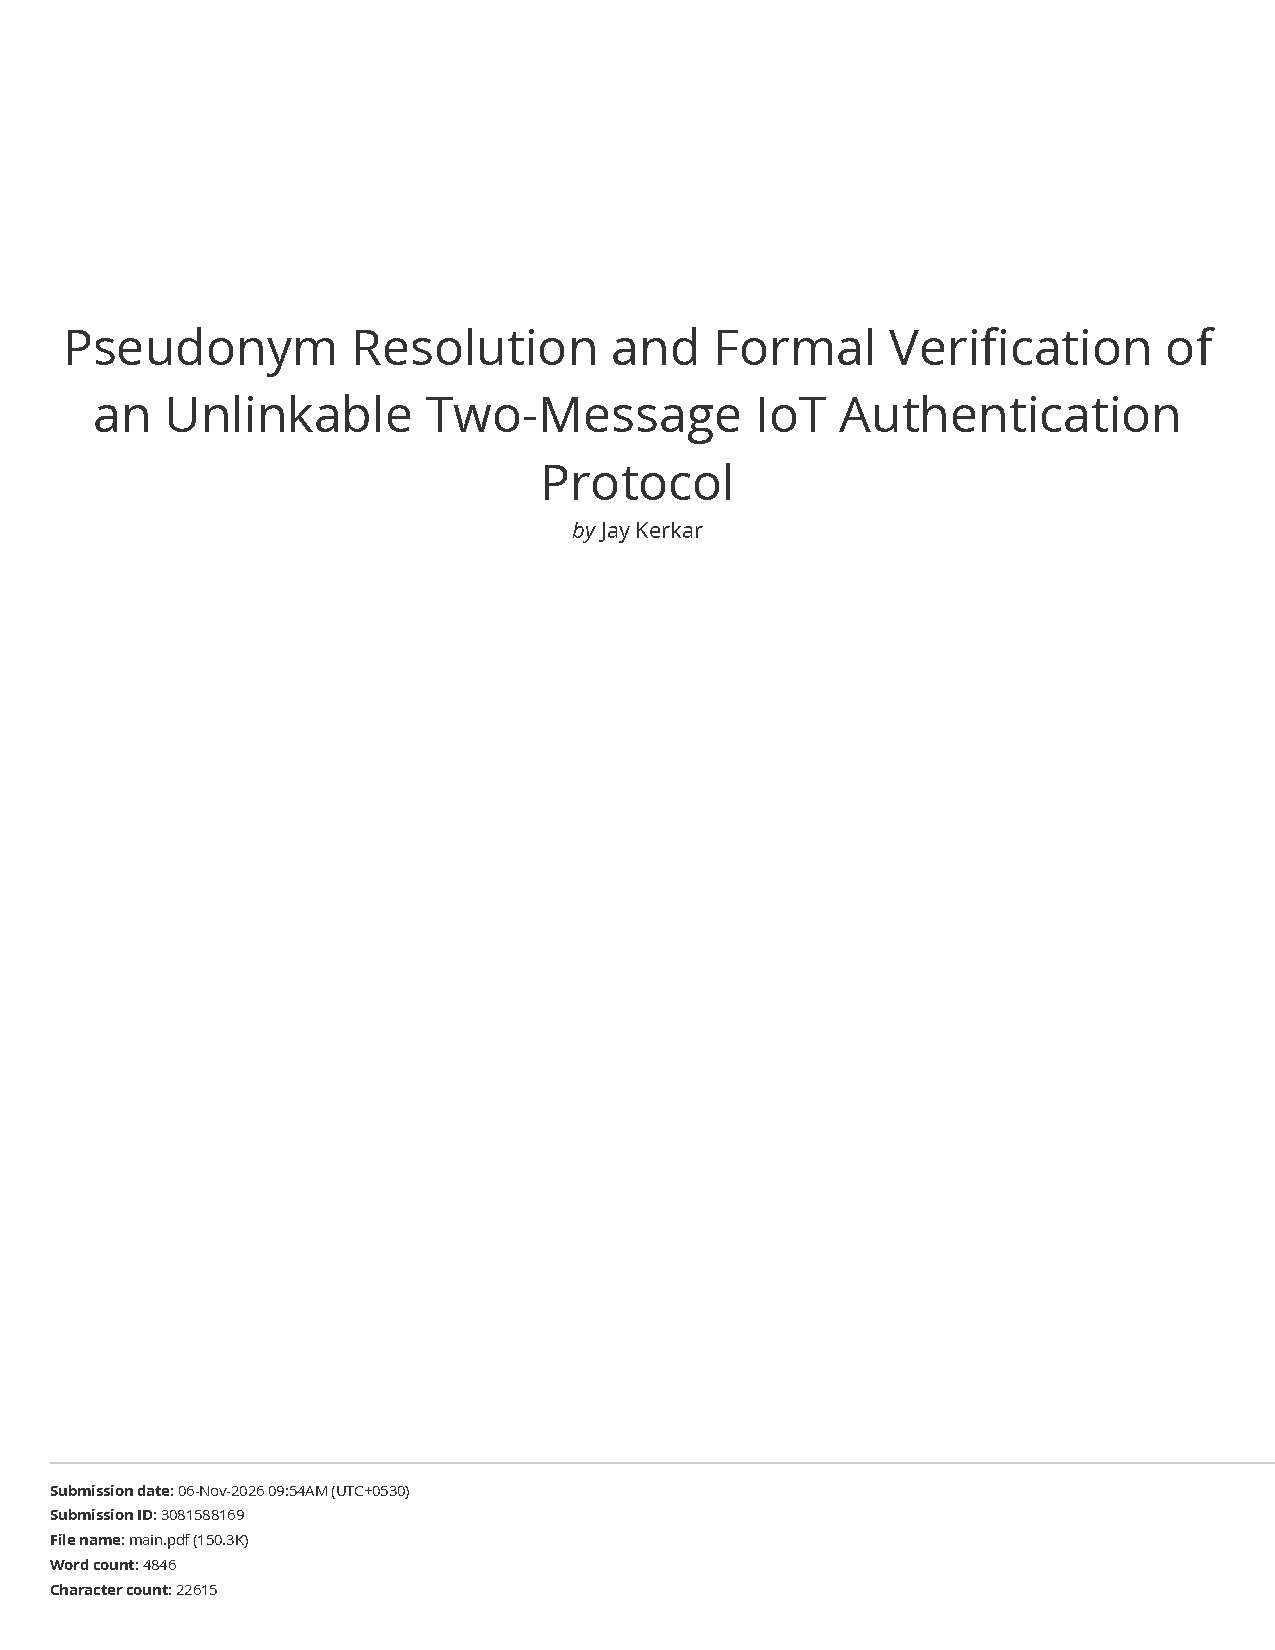
\includepdf[pages=-,scale=0.86,pagecommand={\thispagestyle{bb}}]{reports/plagiarism_report.pdf}

\subsection*{AI writing detection report}
The same paper was also checked with Turnitin's AI writing detection (Submission ID \texttt{trn:oid:::1:3711052702}, 14~November 2026). The report shows no AI-writing score, since scores below the 20\% threshold are not surfaced by the tool. The report is reproduced on the following pages.

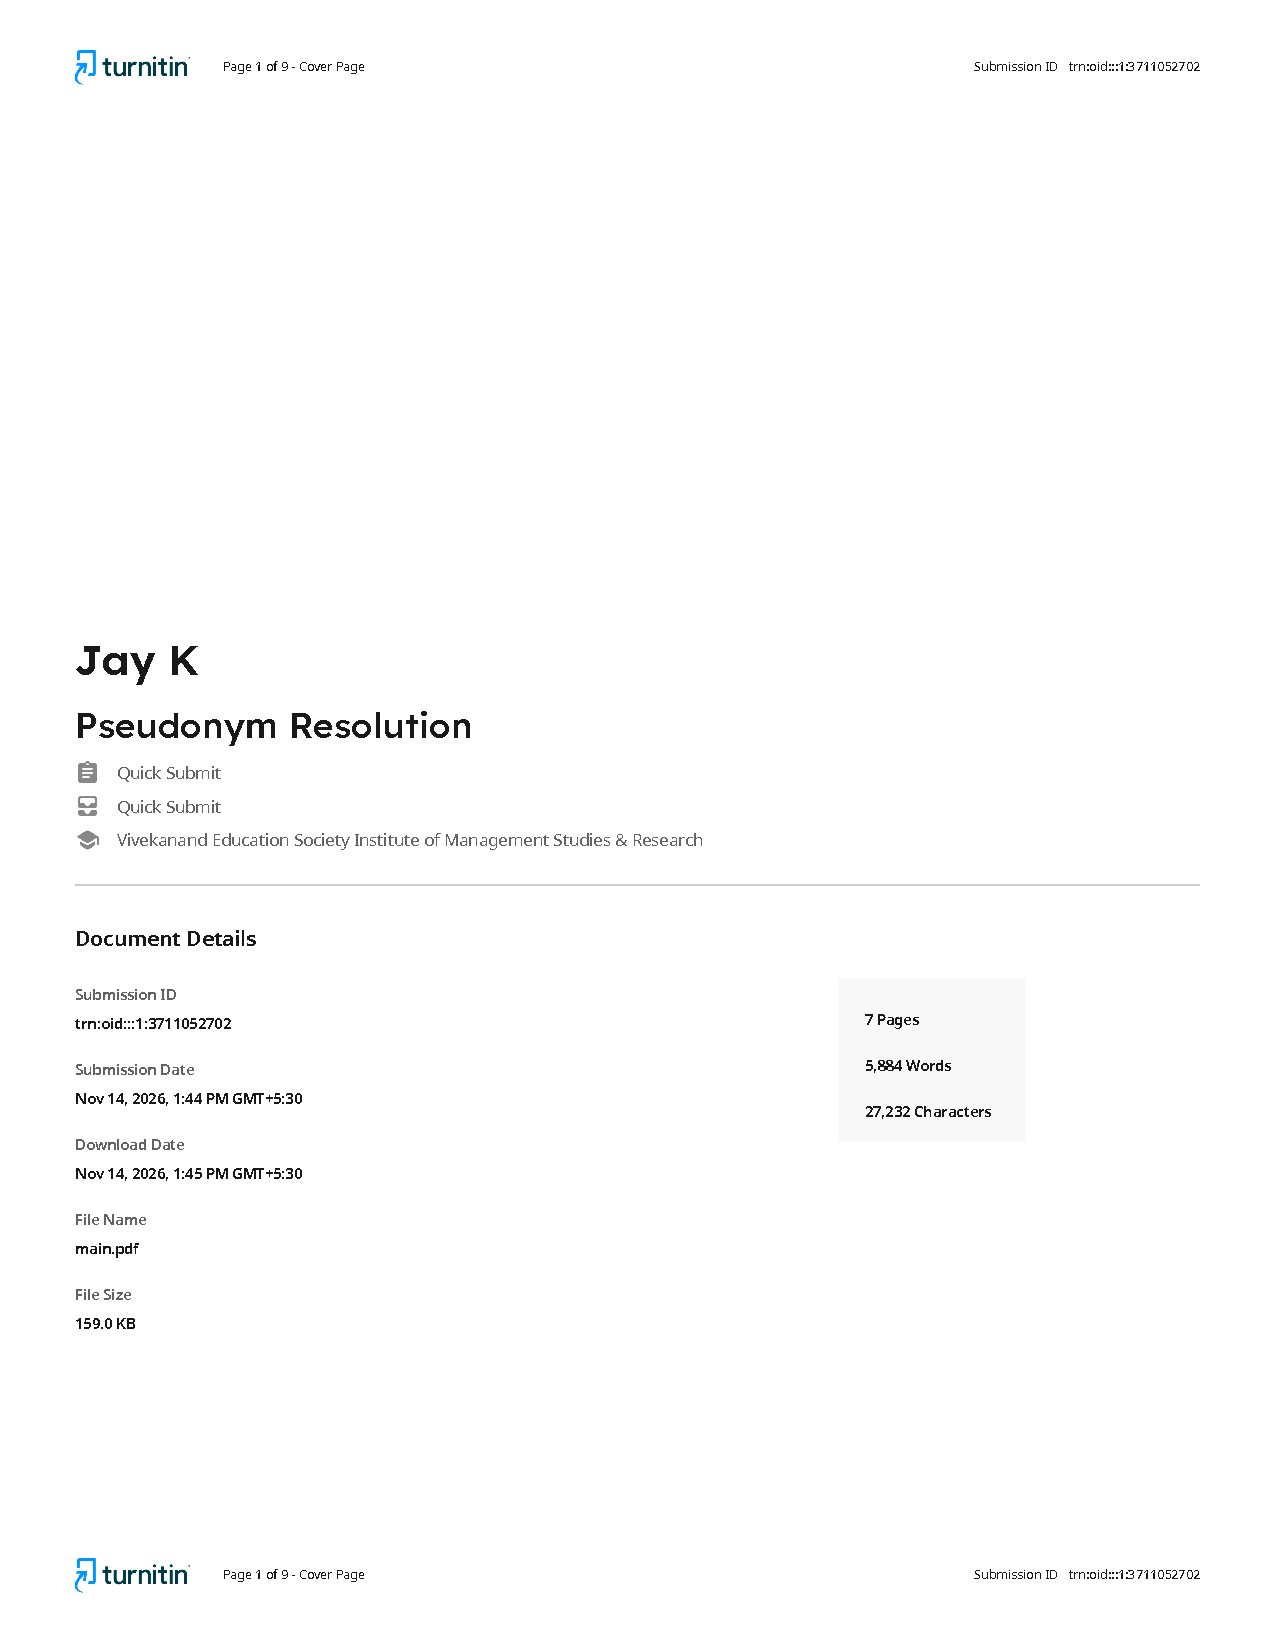
\includepdf[pages=-,scale=0.86,pagecommand={\thispagestyle{bb}}]{reports/ai_detection_report.pdf}

\section*{A.II. IPR: Copyright/Patent/etc. (if granted)}
\addcontentsline{toc}{section}{A.II. IPR: Copyright/Patent/etc.}
The copyright registration application for the project's codebase is being prepared. Application and registration details will be added when available. The software is released under the Apache License~2.0, copyright 2026 Jay Kerkar, Chaitanya Kelkar, Chirag Poornamath, Yash Kolekar and Shanta Sondur.
